%----------------------------------------------------------------------------
\chapter{A generált monitor forráskód helyességének tesztelése}
%----------------------------------------------------------------------------

%----------------------------------------------------------------------------
\section{Tesztelési célok}
%----------------------------------------------------------------------------

A generált monitor forráskód tesztelésére a következő célokat fogalmazuk meg:

\begin{itemize}
    \item Az összes üzenet típus megjelenése a különböző teszt szenáriókban
    \item Időzített feltételek helyes kiértékelése
    \item Üzenet megkötések tesztelése
    \item Alt és Par operátorok esetén, az üzenet szekvencia ágak helyes kiértékelése
    \item Loop operátor esetén a minimális és maximálás üzenet ismétlődések tesztelése
    \item Összetett szenárió tesztelése, ami több operátort tartalmaz
    \item Egymást követő elvárt üzeneteket tartalmazó szenárió tesztelése
    \item Egymást követő fail üzeneteket tartalmazó szenárió tesztelése
    \item Regular üzenet tesztelése (ha megjelenik a rendszer működésében akkor ki kell értékelni a szenárió többi részét, ha nem jelenik meg a monitor helyes működést kell jelezzen és, hogy a követelmény nem teljesült)
    \item Több óraváltozót tartalmazó szenárió tesztelése
    \item Egymást követő üzenetek kombinációinak tesztelése (pl. elvárt üzenetet követő fail, elvárt üzenetet követő reguláris, stb.)
\end{itemize}

%----------------------------------------------------------------------------
\clearpage\section{Monitor forráskód generátor tesztelése}
%----------------------------------------------------------------------------

A generált monitor forráskodját integrációs tesztek segítségével szeretnénk tesztelni.
A teszteinkben egy példa rendszer java implementációját integráljuk a generált monitor komponenssel.
Az Xtext keretrendszer a specifikált DSL (Domain Specific Language) nyelvhez generál egy Maven plugin-t.
Ezt a plugin-t betölthetjük egy egyszerű maven projektbe és használhatjuk is az elkészített DSL nyelvünket, azaz létrehozhatunk a projektben a saját DSL-ünkhöz tartozó fájlokat, melyekben megadhatjuk saját scenario-inkat.

\begin{figure}[!ht]
    \centering
    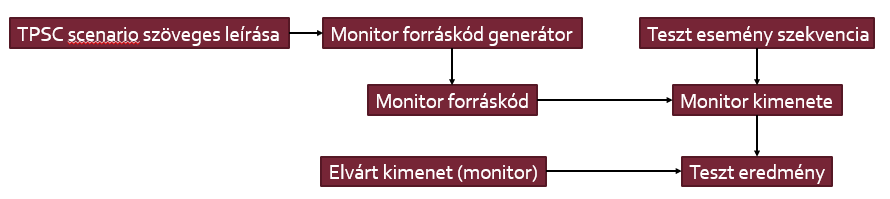
\includegraphics[width=150mm, height=9cm, keepaspectratio]{figures/integration_test_flow.png}
    \caption{Integrációs tesztelés folyamatábrája.}
\end{figure}

A 9.2. ábrán megtekinthető az integrációs tesztelés tervének folyamatábrája.
A következők tesztelési kategoriáink:

\begin{itemize}
    \item Scenario operátorok tesztelése
    \item Üzenet paraméterek tesztelése
    \item Időzítések tesztelése
\end{itemize}

A scenario operátorok tesztelésénél az a célunk, hogy a monitor a követelmény különböző ágait figyelembe véve helyes kimenetet adjon.
Például loop operátor esetén a minimum, köztes és maximum üzenet szekvencia ismétléseknél is helyes legyen a monitor kimenete.
Ha a maximumnál többször szerepel az üzenet szekvencia akkor hibát kell, hogy jelezen.
Üzenet paraméterek tesztelése esetén azt szeretnénk vizsgálni, hogy a monitor helyesen értelmezi e az üzenet paramétereket.
Az időzítések tesztelésénél az a fontos, hogy a monitor képes-e az óraváltozók alapján az időzitési feltételeket kiértékelni.
Például ha az üzenet a feltétel alapján időben érkezik meg akkor helyes kimenetet adjon vissza ha feltétel szerint később érkezik meg akkor a monitornak hibát kell jeleznie.

Egy integrációs teszt akkor sikeres ha a monitor kimenete megegyezik az elvárt kimenettel.
Az elvárt kimenetet a rendszer manuális tesztelése határoz meg.
A tesztelő dönti el, hogy helyesen kell hogy működjön vagy sem amit a monitornak jeleznie kell.

%----------------------------------------------------------------------------
\clearpage
%----------------------------------------------------------------------------

Az Xtext keretrendszer a definiált DSL nyelvünkhöz generál egy Maven projekt architektúrát.
A nyelvünk így elérhető maven plugin formájában is, amit felhasználhatunk az integrációs teszteinkhez.
Elég csupán egy maven projektet felkonfigurálni a saját dsl plugin-ünkkel és elkészítethetjük a saját tesztelési keretrendszerünket.
Ezek a maven projektek a szülő projektünkben helyezkedhetnek el, így a projekt struktúrában közvetlen a nyelvünk mellett vannak.
A 9.3. ábrán és a 9.1. kódrészléten látható egy ilyen integrációs teszthez tartozó maven projekt felépítése és a hozzá tartozó teszteset.

\begin{figure}[!ht]
    \centering
    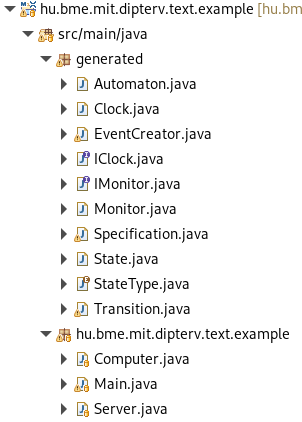
\includegraphics[width=150mm, height=9cm, keepaspectratio]{figures/integration_test_structure.png}
    \caption{Példa integrációs teszt projekt struktúrája.}
\end{figure}

A 9.3. ábrán lévő \textit{generated} csomag tartalmazza a scenariohoz tartozó generált automata forráskódját és a monitor forráskódját.
A \textit{hu.bme.mit.dipterv.text.example} csomag a tesztelt rendszer \textit{Java} implementációját tartalmazza.

\begin{lstlisting}[language=java, frame=single, float=ht!, caption={Integrációs teszteset.},captionpos=b]
package hu.bme.mit.dipterv.text.example;

import org.junit.jupiter.api.Test;
import org.junit.jupiter.api.Assertions;

import generated.Specification;
import generated.IClock;
import generated.IMonitor;
import generated.Monitor;
import generated.Clock;

public class MonitorPassingTest {

	@Test
	public void testMonitorPassing() {
		Specification specification = new Specification();
		specification.listAutomatas();
		IClock clock = new Clock();
		IMonitor monitor = new Monitor(specification.getAutomata().get(0), clock);

		Server server = new Server(monitor);
		Computer computer = new Computer(server, monitor);
		Assertions.assertTrue(monitor.goodStateReached());
	}
}
\end{lstlisting}

\begin{lstlisting}[language=java, frame=single, float=ht!, caption={Integrációs teszteset eredménye.},captionpos=b]
-------------------------------------------------------
T E S T S
-------------------------------------------------------
Running hu.bme.mit.dipterv.text.example.MonitorPassingTest
q0 NORMAL
q1 NORMAL
q2 ACCEPT
q3 NORMAL
q4 NORMAL
q5 FINAL
!(computer.checkEmail().computer) q0->q0
computer.checkEmail().computer q0->q1
!(computer.sendUnsentEmail().server) q1->q1
!(computer.sendUnsentEmail().server) q1->q2
computer.sendUnsentEmail().server q1->q3
!(computer.logout().server) & !(computer.newEmail().server) q3->q3
computer.newEmail().server q3->q4
!(computer.downloadEmail().server) q4->q4
computer.downloadEmail().server q4->q5
Received Message: computer.checkEmail().computer
Transition: !(computer.checkEmail().computer)
Transition: computer.checkEmail().computer
transition triggered: computer.checkEmail().computer
q1

Received Message: computer.sendUnsentEmail().server
Transition: !(computer.sendUnsentEmail().server)
Transition: !(computer.sendUnsentEmail().server)
Transition: computer.sendUnsentEmail().server
transition triggered: computer.sendUnsentEmail().server
q3

Received Message: computer.newEmail().server
Transition: !(computer.logout().server) & !(computer.newEmail().server)
Transition: computer.newEmail().server
transition triggered: computer.newEmail().server
q4

Received Message: computer.downloadEmail().server
Transition: !(computer.downloadEmail().server)
Transition: computer.downloadEmail().server
transition triggered: computer.downloadEmail().server
q5

Tests run: 1, Failures: 0, Errors: 0, Skipped: 0, Time elapsed: 0.025 sec

Results :

Tests run: 1, Failures: 0, Errors: 0, Skipped: 0
\end{lstlisting}

A 9.2. kódrészlet a Maven teszt kimenetét tartalmazza.

Ezt a projekt struktúrát felhasználva a teszteink köré tudunk egy Maven alapú Continuous Integration-t (CI) állítani.

A függelékben található egy példa unit teszt eset az automata generátor tesztelésére.

%----------------------------------------------------------------------------
\clearpage\section{Continuous Integration}\subsection{Github Actions CI}
%----------------------------------------------------------------------------

Az időzített automata és monitor forráskód generátorok automatikus tesztelése a Github Actions segítségével történik.
A CI minden feltöltött új commit esetén lefut.
A CI különböző fázisai a következők:

\begin{itemize}
    \item I. Teljes Xtext projekt fordítása (Maven)
    \item II. Intergrációs tesztek futtatása
\end{itemize}

A generátorokhoz tartozó Xtext projekten lefut egy Maven build, amely az új feltöltött verzió tartalmazza.
Ez a build állítja elő a DSL nyelvhez tartozó Maven plugin-t is.
A fordítással együtt lefutnak a unit tesztek is.
Ezt követően hajtódnak végre az integrációs tesztek, amelyek a frissen fordított Maven plugint használják.
Ha az összes fázis sikeresen lefutott, akkor az adott commit nem rontott el semmilyen korábbi funkciót.
A CI-hoz tartozó script-et a 9.3. kódrészlet tartalmazza.

\begin{figure}[!ht]
    \centering
    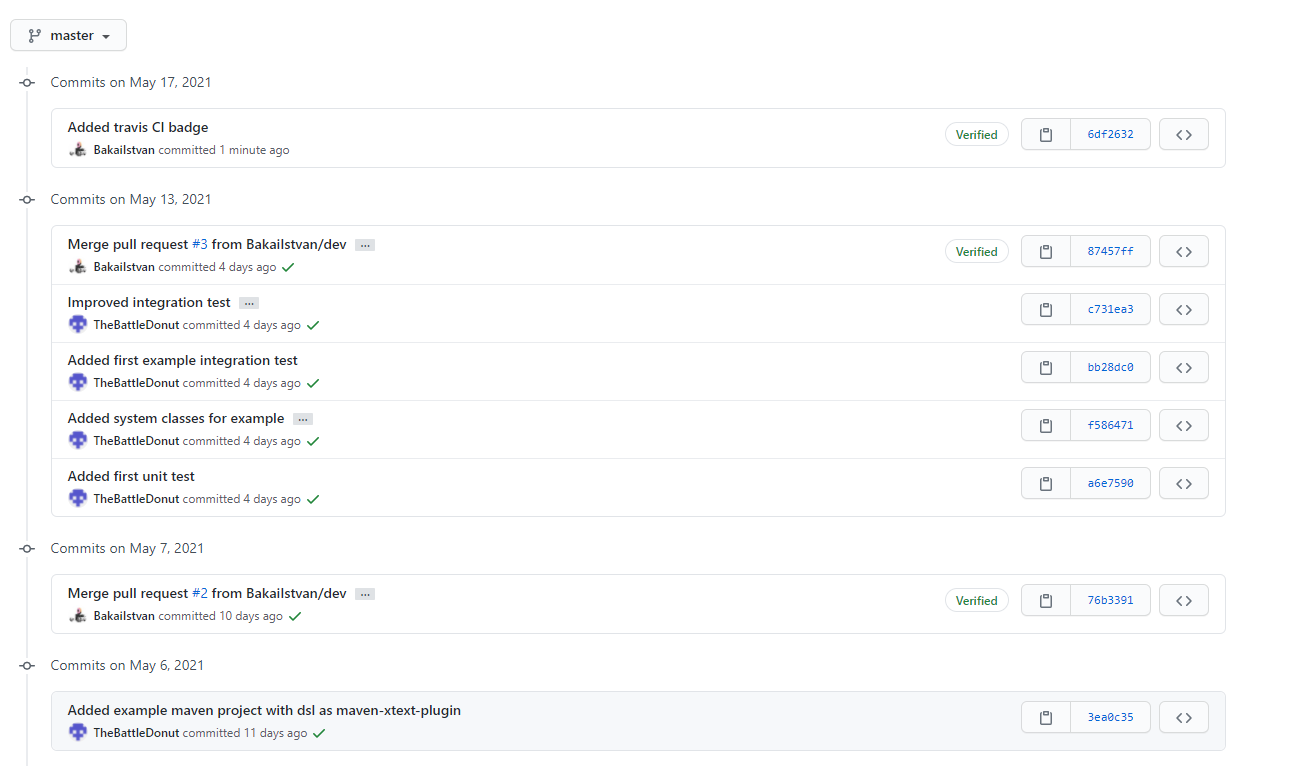
\includegraphics[width=150mm, keepaspectratio]{figures/github_ci_check.png}
    \caption{GitHub repository commit-ok és hozzá tartozó CI check-ek.}
\end{figure}

\begin{figure}[!ht]
    \centering
    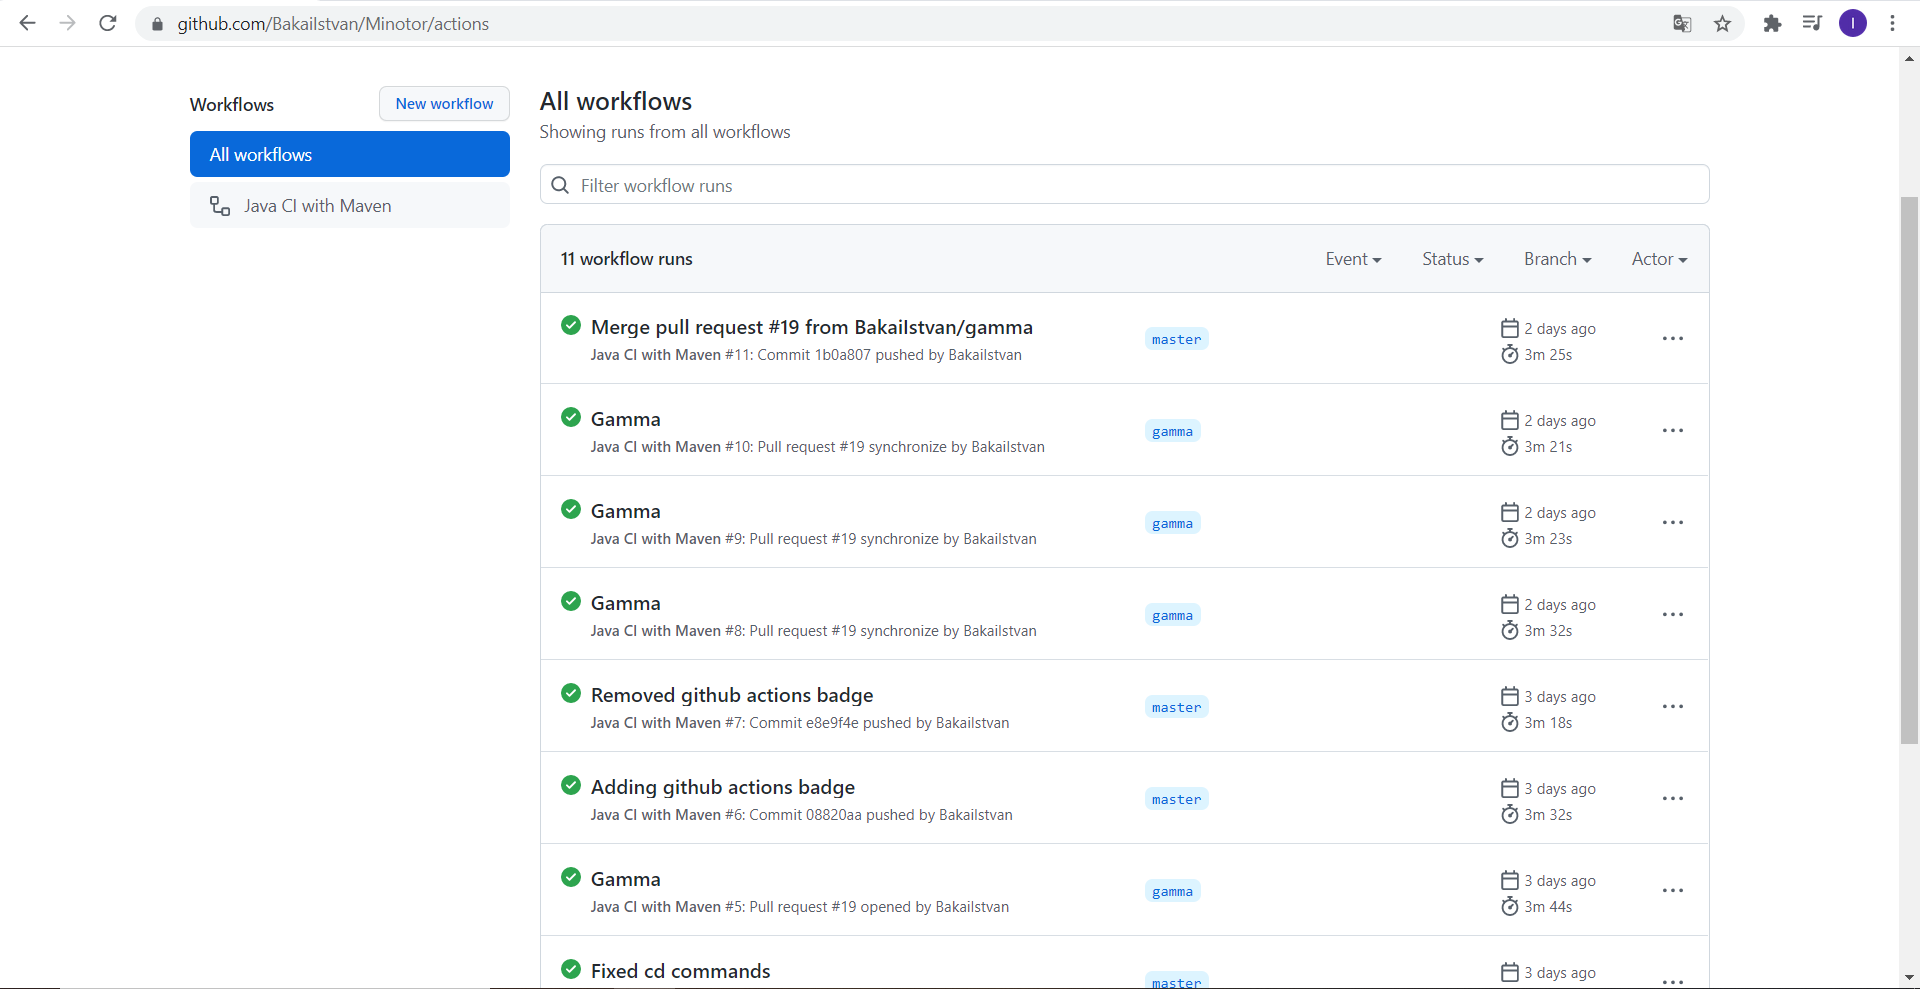
\includegraphics[width=150mm, keepaspectratio]{figures/github_ci_builds.png}
    \caption{Github Actions CI build-ek eredményei.}
\end{figure}

\begin{lstlisting}[language=java, frame=single, float=ht!, caption={Github Actions CI-hoz tartozó .yml script.},captionpos=b]
# This workflow will build a Java project with Maven, and cache/restore any dependencies to improve the workflow execution time
# For more information see: https://help.github.com/actions/language-and-framework-guides/building-and-testing-java-with-maven

name: Java CI with Maven

on:
    push:
    branches: [ master ]
    pull_request:
    branches: [ master ]

jobs:
    build:

    runs-on: ubuntu-latest

    steps:
    - uses: actions/checkout@v2
    - name: Set up JDK 11
        uses: actions/setup-java@v2
        with:
        java-version: '11'
        distribution: 'adopt'
        cache: maven
    - name: Build with Maven
        run: mvn clean install -U
    - name: Test example project
        run: cd hu.bme.mit.dipterv.text.example; mvn clean install -U
    - name: Test mobileexample project
        run: cd hu.bme.mit.dipterv.text.mobileexample; mvn clean install -U
    - name: Test altexample project
        run: cd hu.bme.mit.dipterv.text.altexample; mvn clean install -U
    - name: Test parexample project
        run: cd hu.bme.mit.dipterv.text.parexample; mvn clean install -U
    - name: Test operatorexample project
        run: cd hu.bme.mit.dipterv.text.operatorexample; mvn clean install -U
    - name: Test gamma integration project
        run: cd hu.bme.mit.dipterv.text.gammaexample; mvn clean install -U
\end{lstlisting}

%----------------------------------------------------------------------------
\clearpage\section{Tesztesetek}\subsection{Egyszerű időzítési megkötéseket tartalmazó tesztszenárió}
%----------------------------------------------------------------------------

A tesztesetekhez tartozó scenario követelmény megtalálható az x. ábrán.

\begin{lstlisting}[language=java, frame=single, float=ht!, caption={Integrációs teszteset.},captionpos=b]
specification Email {

	object Computer computer;
	object Server server;

	integer timeout = 10;
	string receiver = "John";
	string subject = "Next meeting";

	clock x;

	constraint constraints {
		message logout() computer -> server;
	}

	scenario sendEmail{
		message checkEmail() computer -> computer reset x;
		required message sendUnsentEmail() computer -> server;
		pastConstraint {constraints} message newEmail(receiver, subject) computer -> server;
		message downloadEmail(timeout) computer -> server clockConstraint {>(x,10)};
	}
}
\end{lstlisting}

\begin{figure}[!ht]
    \centering
    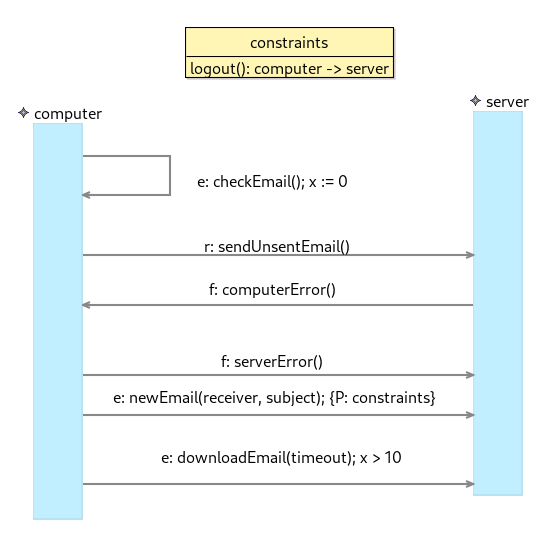
\includegraphics[width=150mm, keepaspectratio]{figures/diagramExample.png}
    \caption{Szenárió diagram.}
\end{figure}

A rendszerben egy szervergépből és egy felhasználói számitogépből áll.
A szerver egy e-mail szervert szimulál, aminek a számitogép különböző kéréseket küldhet.
Például lekérdezheti tőle a kapott e-mail vagy új e-mail küldhet.
A követelményben leírjuk, hogy a rendszernek mi a helyes viselkedése e-mail küldés esetén.
Ha a computer a \textit{checkEmail} hívást használva talál elküldendő e-mail az továbbítja a szervernek.
Ezt az \textit{elvárt} \textit{sendUnsentEmail} üzenet jelzi.
Ezt követően meg kell jelenjen a rendszer működésében a \textit{newEmail} üzenet.
A ehelyett \textit{logout} üzenet érkezik a hibás működést jelent.
A \textit{newEmail} üzenetet a \textit{downloadEmail} üzenet követi.
Ezen az üzeneten van egy 10 másodperces időzítési feltétel, ami a letöltést szimulálja.

A szenárióhoz tartozó tesztesetek a következők:

\begin{itemize}
    \item testNetworkRequirementSatisfied
    \item testNetworkNoErrors
    \item testNetworkWithErrors
    \item testNetworkWithNoDelay
    \item testNetworkFirstFail
    \item testNetworkSecondFail
\end{itemize}

A \textit{testNetworkRequirementSatisfied} tesztesetben a rendszer helyes működését szimuláljuk és azt ellenőrizzük, hogy a generált monitor képes ezt érzékelni és jelzi.
A \textit{testNetworkNoErrors} azt vizsgálja, hogy a monitor képes-e érzékelni, hogy a rendszer nem felelt meg a követelménynek.
Itt úgy manipuláljuk a teszt rendszer, hogy lehagyjuk a letöltés részt a működésből.
Ilyenkor a rendszer nem felel meg a követelménynek, viszont még jó állapotban marad, mert nem történt hiba.
A \textit{testNetworkWithErrors} tesztesetnél a \textit{sendUnsentEmail} üzenet után egy \textit{logout} üzenetet küldünk a monitor és azt vizsgáljuk képes-e detektálni ezt a hibát.
A \textit{testNetworkWithNoDelay}-nél pedig túl gyorsan küldjük a működés végén a \textit{downloadEmail} üzenetet és azt ellenőrizzük képes e a monitor ezt a hibát érzékelni.

%----------------------------------------------------------------------------
\clearpage\subsection{Többféle üzenetet és megkötést tartalmazó egyszerű tesztszenárió}
%----------------------------------------------------------------------------

\begin{lstlisting}[language=java, frame=single, float=ht!, caption={Integrációs teszteset.},captionpos=b]
    specification Photo{

        object User user;
        object Device device;
        object Database db;

        clock x;

        constraint error {
            message closeApp() user -> device;
        }

        scenario playlist_generation{
            message openApp() user -> device reset x;
            message accessWebcam() device -> device clockConstraint {<=(x, 5)} reset x;
            required futureConstraint {error} message getPhoto() device -> user;
            fail message cameraOffline() user -> device;
            required strict message retrieveMood() device -> db;
            required message retrieveMusic() device -> db;
            strict message generatePlaylist() db -> device clockConstraint {<(x, 15)};
        }
    }
\end{lstlisting}

\begin{figure}[!ht]
    \centering
    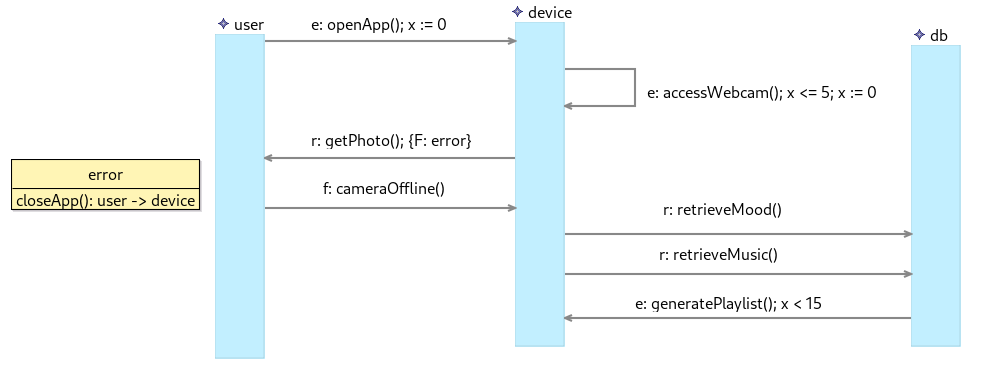
\includegraphics[width=150mm, keepaspectratio]{figures/diagramMobileExample.png}
    \caption{Szenárió diagram.}
\end{figure}

A tesztrendszerünk egy zene lista generáló alkalmazás, ami egy felhasználót, mobileszközt és adatbázist tartalmaz.
A felhasználó "kedve" alapján generálja a listát, amit az arc kifejezése alapján határoz meg.
A követelményben a rendszer alap működése van leírva egészen az elejétől, amikor a felhasználó megnyítja az alkalmazást.
A követelmény leírás megtekinthető az x. ábrán.

A szenárióhoz tartozó tesztesetek a következők:

\begin{itemize}
    \item testMobileRequirementSatisfied
    \item testMobileFutureConstraint
    \item testMobileFutureConstraintEarly
    \item testMobileWithError
    \item testMobileWithDelay
    \item testMobileWithTooMuchDelay
    \item testMobileMissingRequiredMessage
    \item testMobileRequiredEventually
    \item testMobileRequiredNotReceived
\end{itemize}

A teszteseteket a monitor hiba detektáló képeségét tesztelik.
A \textit{testMobileWithDelay} és \textit{testMobileWithTooMuchDelay} tesztesetek az \textit{x <= 5} időzítési feltétel beteljesülését ellenőrzik.
A \textit{testMobileWithDelay} 5 másodperces késleltetéssel küldjük az \textit{accessWebcam} üzenetet, míg a másiknál 6 másodperces késleltetéssel.
Az első esetben a monitornak helyes működést kell érzékelnie a következőben pedig hibás működést.

%----------------------------------------------------------------------------
\clearpage\subsection{Alt operátort tartalmazó tesztszenárió}
%----------------------------------------------------------------------------

A tesztszenárióhoz tartozó rendszerünk egy banki rendszer.
A szenárió megtalálható az x. ábrán.

\begin{lstlisting}[language=java, frame=single, float=ht!, caption={Integrációs teszteset.},captionpos=b]
specification Bank {

    object UserInterface ui;
    object ATM atm;
    object BankDB db;

    bool success = true;

    constraint b {
        message logout() ui->atm;
    }

    scenario transaction {
        message login(success) ui->atm;

        alt (equals(success, true)) {
            pastConstraint {b} message wReq() ui->atm;
            message uDB() atm->db;
        } (equals(success, false)) {
            message loginUnsuccessful() ui->atm;
            required message lockMachine() atm->ui;
        }
    }
}
\end{lstlisting}

\begin{figure}[!ht]
    \centering
    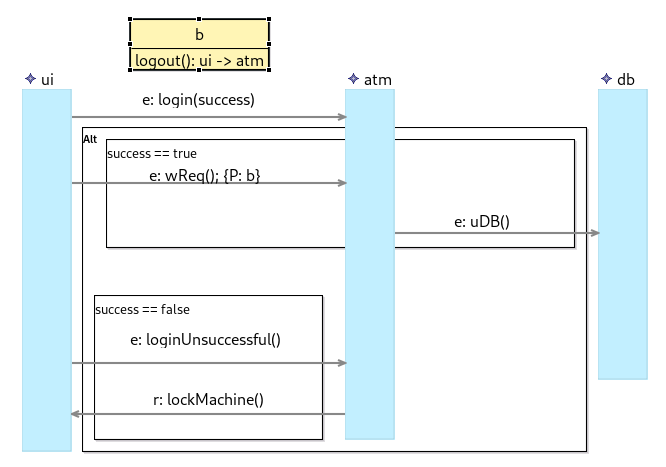
\includegraphics[width=150mm, keepaspectratio]{figures/diagramAltExample.png}
    \caption{Szenárió diagram.}
\end{figure}

A rendszer egy felhasználói felületből, ATM-ből és banki adatbázisból áll.
A követelményünkben két lehetséges működést írunk le.
A \textit{success} paraméter jelzi, hogy melyik működés a helyes.
A szenárióhoz tartozó tesztesetek a következők:

\begin{itemize}
    \item testBankMonitorPassing
    \item testBankMonitorFailing
    \item testBankMonitorFalseCasePassing
    \item testBankMonitorFalseCaseFailing
\end{itemize}

A tesztesetekkel azt vizsgáljuk, hogy a monitor képes-e a helytelen ág lefutását hibának érzékelni és a helyes viselkedés esetén detektálni a követelmény teljesítését.

%----------------------------------------------------------------------------
\clearpage\subsection{Par operátort tartalmazó tesztszenárió}
%----------------------------------------------------------------------------

\begin{lstlisting}[language=java, frame=single, float=ht!, caption={Integrációs teszteset.},captionpos=b]
specification Email {
    object Computer computer;
    object Server server;

    constraint constraints{
        message logout() computer -> server;
    }

    scenario email {
        par {
            case checkEmail {
                message checkEmail() computer -> computer;
            }

            case newEmail {
                pastConstraint {constraints} message newEmail() computer -> server;
            }
        }
    }
}
\end{lstlisting}

\begin{figure}[!ht]
    \centering
    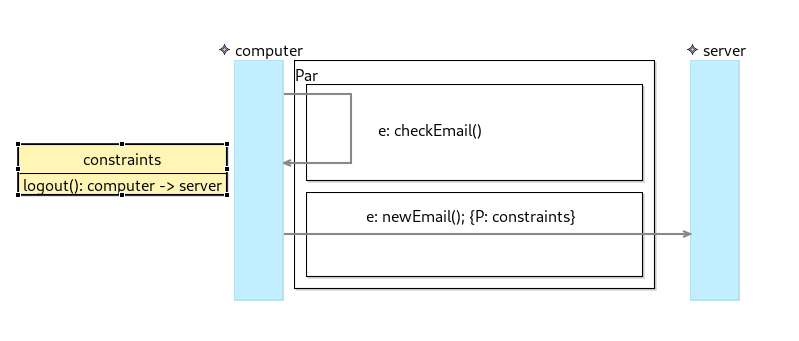
\includegraphics[width=150mm, keepaspectratio]{figures/diagramParExample.png}
    \caption{Szenárió diagram.}
\end{figure}

Ehhez a tesztszenárióhoz az első szenárióban lévő teszt rendszert használtuk fel.
A szenárióhoz tartozó tesztesetek a következők:

\begin{itemize}
    \item testNetworkRequirementSatisfied
    \item testNetworkOtherRequirementSatisfied
\end{itemize}

Azt vizsgáljuk, hogy a monitor képes mindkét permutáció esetén érzékelni a követelmény teljesítését.

%----------------------------------------------------------------------------
\clearpage\subsection{Komplex tesztszenárió loop és alt operátorokkal}
%----------------------------------------------------------------------------

\begin{lstlisting}[language=java, frame=single, float=ht!, caption={Integrációs teszteset.},captionpos=b]
specification Connection {

    object Computer computer;
    object Server server;

    string receiver = "John";
    string subject = "Next Meeting";
    bool success = false;

    clock x;
    clock y;

    constraint logout {
        message logout() computer -> server;
    }

    constraint delete {
        message deleteEmail(subject) computer -> server;
    }

    scenario authentication {
        loop (1, 3) {
            message login() computer -> computer reset x;
            pastConstraint {logout} message attemptLogin() computer -> server reset y;
        }

        alt (equals(success, true)) {
            message checkEmail() computer -> server clockConstraint {<(x, 2)};
            required futureConstraint {delete} message newEmail(receiver, subject) computer -> server reset x;
        } (equals(success, false)) {
            required message logoutUser() server -> computer clockConstraint {>(y, 3)};
            message lockComputer() server -> computer reset y;
        }
    }
}
\end{lstlisting}

\begin{figure}[!ht]
    \centering
    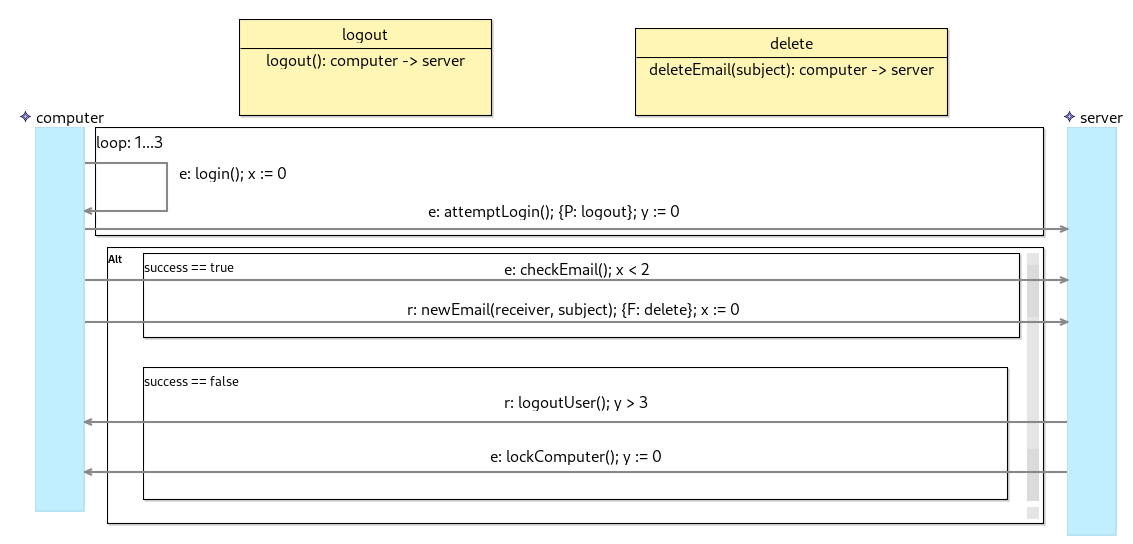
\includegraphics[width=150mm, keepaspectratio]{figures/diagramOperatorExample.png}
    \caption{Szenárió diagram.}
\end{figure}

\begin{itemize}
    \item testNetworkRequirementSatisfied
    \item testNetworkRequirementSatisfiedTwice
    \item testNetworkRequirementSatisfiedThreeTimes
    \item testNetworkRequirementSatisfiedFourTimes
    \item testNetworkAltTrueCase
    \item testNetworkAltTrueCaseSatisfied
    \item testNetworkLogoutTooFast
    \item testNetworkLogoutConstrait
\end{itemize}

\clearpage\section{Tesztelés összefoglaló}

\begin{longtable}{|p{0.1428\linewidth}|p{0.1428\linewidth}|p{0.1428\linewidth}|p{0.1428\linewidth}|p{0.1428\linewidth}|p{0.1428\linewidth}|}
\hline
\textbf{Tesztelési célok} & \textbf{Egyszerű tesztszenárió} & \textbf{Több üzenetet tartalmazó tesztszenárió} & \textbf{Alt operátort tartalmazó tesztszenárió} & \textbf{Par operátort tartalmazó tesztszenárió} & \textbf{Komplex tesztszenárió}\\
\hline
Egyszerű üzenet megjelenése & X & X & X & X & X\\
\hline
Elvárt üzenet megjelenése & X & X & X & - & X\\
\hline
Nem kivánt (fail) üzenet megjelenése & X & X & - & - & -\\
\hline
Strict üzenet tesztelése & - & X & - & - & -\\
\hline
Időzítési feltételek tesztelése & X & X & - & - & X\\
\hline
Past megkötés tesztelése & X & - & X & X & X\\
\hline
Future megkötés tesztelése & - & X & - & - & X\\
\hline
Alt operátor tesztelése & - & - & X & - & X\\
\hline
Par operátor tesztelése & - & - & - & X & -\\
\hline
Loop operátor tesztelése & - & - & - & - & X\\
\hline
Több operátort tartalmazó szenárió tesztelése & - & - & - & - & X\\
\hline
Egymást követő elvárt üzenetek & - & X & - & - & -\\
\hline
Egymást követő fail üzenetek & X & - & - & - & -\\
\hline
Sima üzenet tesztelése & X & X & X & X & X\\
\hline
Több óraváltozó & - & - & - & - & X\\
\hline
Elvárt után fail üzenet & X & - & - & - & -\\
\hline
Fail után elvárt üzenet & - & X & - & - & -\\
\hline
\caption{Összefoglaló táblázat}
\label{tab:table1}
\end{longtable}